\section{مرور}

در دو جلسه اخیر با گراف و دو طریق نگهداری آن (ماتریس و لیست مجاورت) آشنا شدیم و دو راه برای پیمایش آن یاد گرفتیم (جستجوی اول سطح و اول عمق). در این جلسه به پیاده سازی این دو الگوریتم می‌پردازیم و شباهت‌هایشان را خواهیم دید.

فرض کنیم که ما می‌خواهیم یک گراف را پیمایش کنیم. در جستجوی اول سطح با شروع از یک گره و ملاقات آن کلیه گره‌های مجاور آن نیز ملاقات می‌شوند. این روند برای نقاط همسایه نیز تکرار می‌شود. در جستجوی اول عمق از یک نقطه شروع می‌کنیم و پس از ملاقات آن به یک سمت حرکت می‌کنیم. یعنی از آن به راس بعدی رفته و از راس بعدی تا وقتی که درهمسایه‌اش کسی دیده‌ نشده نباشد این روند را ادامه می‌دهیم. آن‌گاه عقب‌ گرد کرده تا به راس اول برسد و الگوریتم تمام شود. جلسه پیش یک پیاده‌سازی هم دیدیم و تحلیل کردیم مرتبه زمانی آن برای گراف با ماتریس از مرتبه $O(V^2)$ می‌شود و با لیست مجاورت از مرتبه $O(V+E)$.

\section{پیاده سازی DFS}

پیشنهاد اول برای این الگوریتم به شکل زیر و به کمک پشته است. 

\begin{figure}[h!]
\centering
\includegraphics[width=75mm]{s1}
\caption{پیاده‌سازی اول}
\label{fig:first_impl}
\end{figure}

اما مشکلی که در این جا وجود دارد این است ممکن است راسی دوبار دیده شود.
\footnote{
توجه کنید آن‌چه که به آن توجه شده است این است که راسی که بررسی می‌کنیم دیده نشده باشد اما ممکن است یک راس پیش از دیده شدن توسط چندین همسایه‌اش به پشته اضافه شود.	
}
 پس ابتدا بررسی می‌کنیم که راس قبلا دیده نشده باشد.


\begin{figure}[h!]
\begin{center}
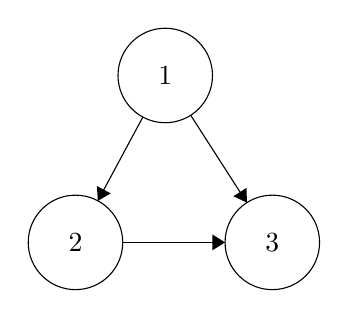
\begin{tikzpicture}[scale=0.2]
\tikzstyle{every node}+=[inner sep=0pt]
\draw [black] (38.4,-17.5) circle (3);
\draw (38.4,-17.5) node {$1$};
\draw [black] (32.7,-28.1) circle (3);
\draw (32.7,-28.1) node {$2$};
\draw [black] (45.2,-28.1) circle (3);
\draw (45.2,-28.1) node {$3$};
\draw [black] (36.98,-20.14) -- (34.12,-25.46);
\fill [black] (34.12,-25.46) -- (34.94,-24.99) -- (34.06,-24.52);
\draw [black] (35.7,-28.1) -- (42.2,-28.1);
\fill [black] (42.2,-28.1) -- (41.4,-27.6) -- (41.4,-28.6);
\draw [black] (40.02,-20.03) -- (43.58,-25.57);
\fill [black] (43.58,-25.57) -- (43.57,-24.63) -- (42.73,-25.17);
\end{tikzpicture}
\end{center}
\caption{
مشکل دوبار دیده شدن. راس ۳ دو بار توسط راس‌های ۱ و ۲ به پشته اضافه می‌شود.
}
\end{figure}

\begin{figure}[b!]
\centering
\includegraphics[width=90mm]{s2}
\caption{پیاده سازی DFS
با پشته
}	
\label{fig:dfs_impl}
\end{figure}

\begin{figure}[t!]
\centering
\includegraphics[width=60mm]{w5}
\caption{
تحلیل زمانی
DFS 
با ماتریس مجاورت 
}
\end{figure}


حال سوال پیش می‌آید که زمان اجرای این الگوریتم در صورت ذخیره گراف به شکل‌های ماتریس یا لیست مجاورت چگونه خواهد 
بود.  ماتریس و لیست مجاورت در زمان اجرای foreach که راس‌های همسایه را نگاه می‌کند تفاوت ایجاد خواهند کرد.

حلقه while به تعداد دفعاتی که در پشته چیزی وارد می‌کنیم اجرا می‌شود و هر راس تنها یک بار از if رد می‌شود
(شکل
~\ref{fig:dfs_impl}
)
 چون تنها بار اولی که هر راس را می‌بینیم visited اش false است.  پس برای هر راس همسایه‌هایش یک بار بیشتر درج نمی‌شود و
 جمعا از$O(E)$ درج انجام می‌شود پس حلقه بیرونی نیز به همین اندازه 
   اجرا خواهد شد. اگر گراف به شکل لیست‌ مجاورت نگهداری شده باشد همسایه‌های رئوس جمعا در 
$O(E)$
  دیده می‌شوند. اما از ماتریس مجاورت استفاده کنیم برای هر راس باید مجاورت داشتنش با همه رئوس دیگر را بررسی کنیم که
$O(V^2)$
    خواهد بود.

پس DFS با ماتریس مجاورت مرتبه زمانی‌اش 
$O(V^2)$
خواهد بود یا 
$O(V^2+E)$
برای وقتی که یال‌های چندگانه داشته باشیم.
اگر الگوریتم را با 
لیست اتصال بزنیم مرتبه 
for 
به جای 
$O(V^2)$
به 
$O(E)$
تبدیل خواهد شد و مرتبه کل از 
$O(V+E)$
خواهد بود.

\paragraph{
شباهت با BFS
}
برای پیاده‌سازی BFS هم می‌توانیم در کد بالا پشته را به صف تبدیل کنیم!

\section{
\lr{
back edge, forward edge, cross edge
}
}

\paragraph{تعریف}
 اگر در درخت جستجوی به دست آمده یک گره به نوه‌‌اش یالی در گراف اصلی داشته باشد به آن 
\lr{forward edge}
  می‌گوییم. اگر یک گره به پدر غیرمستقیم خود (اجداد پدرش) یال داشته باشد 
\lr{back edge}
 داریم و اگر بین دو گره که هیچ کدام جد دیگری نباشد یال داشته باشیم 
\lr{cross edge}
 داریم. 

\paragraph{سوال}
 آیا DFS می‌تواند 
\lr{forward edge}
 داشته باشد؟ بله. 
\lr{back edge}
  چطور؟ بله. 
\lr{cross edge}
چه؟
اگر گراف دوطرفه باشد cross به وجود نمی‌آید. ولی اگر جهت‌دار باشد ممکن است٫ ولی یال‌هایی که هستند از راست به چپ می‌باشند٫ یعنی از کسانی که دیرتر دیده شدند به سمت کسانی که زودتر دیده شدند.

\begin{figure}[b!]
\centering
\includegraphics[width=90mm]{s3.jpeg}
\caption{
از راست به چپ
یال‌های  پیشرو
\lr{(forward edge)}
٫عبوری
\lr{(cross edge)}
}
و
 پشتی(بازگشتی)
\lr{(back edge)}

\end{figure}

\paragraph{سوال}
 توی BFS آیا 
\lr{forward edge}
  داریم؟ نه. 	چون تمام همسایه های یک راس گراف در درخت جستجو BFS مثبت منفی یک اختلاف سطح دارند. ولی 
\lr{back edge}
 اگه گراف جهت دار باشد می‌توانیم داشته باشیم (و در غیر این صورت نه).
\lr{cross edge}
  نیز داریم اما یا هم‌ سطح خود گره٫ یا به سطح قبلی و یا بعدی.

\section{
کاربرد های DFS و BFS
}
BFS نزدیک ترین فاصله راس ها تا راس ما رو میده (شماره سطر ها همان فاصله می‌شوند).
 و از
DFS
برای پیدا کردن دور در گراف می‌توان استفاده کرد.
یک کاربرد دیگر این دو الگوریتم را در جلوتر می‌بینیم.

\subsection{connectivity}

حال درباره اتصال
\footnote{connectivity}
 صحبت می‌کنیم.

\paragraph{تعریف اتصال}
در گراف بدون جهت دو راس که به هم مسیر دارند را 
\textit{متصل} 
\footnote{connected}
می‌گوییم.

\paragraph{تعریف مولفه هم‌بندی}
مجموعه‌ راس‌هایی که هر دو راس آن به هم مسیر دارند و از هیچ راس خارج از این مجموعه به آن‌ها مسیری نباشد یک 
\textit{
مولفه هم‌بندی
}
\footnote{\lr{connected component}}
تشکیل می‌دهند.

با پیدا کردن مولفه‌های هم‌بندی گراف را می‌توان به یک سری زیر گراف شکست که به هم هیچ یالی ندارند.
پیدا کردن مولفه‌های همبندی با هر دو الگوریتم
BFS
و 
DFS
امکان‌پذیر است.
کافی است یک حلقه بالای الگوریتم‌‌های مطرح شده (
شکل 
\ref{fig:dfs_impl}
)
اضافه کنیم برای کامپوننت‌های مختلف.
پیمایش با شروع از هر راس که تمام شود در پایانش یک مولفه‌همبندی (شامل آن راس) را می‌دهد.

در گراف جهت‌دار بین دو مولفه هم‌بندی می‌تواند یال (تنها از سمت یک مولفه) هم باشد. 
(شکل \ref{two_comp}
)
البته در آن‌جا مولفه قویا هم‌بندی
\footnote{\lr{strongly connected component}}
 گفته می‌شود.

\begin{wrapfigure}{r}{50mm}
%  \begin{center}
    \includegraphics[width=35mm]{components.png}
    \label{two_comp}
%	 \end{center}
	 \caption{
	 دو مولفه قویا هم‌بندی
	 \\
	  و یال بین آن دو
	 }
\end{wrapfigure}

%\begin{figure}[h]
%	\includegraphics[width=50mm]{components}
%	\label{two_comp}
%	\caption{دو مولفه قویا هم‌بندی}
%\end{figure}

فرض کنید مولفه های هم‌بندی مختلف داریم.
حال اگر به جای رأس‌ها به مولفه‌های هم‌بندی نگاه کنیم می‌توان گراف را منقبض کرد. هر یالی که از راس‌های انقباض به بیرون است بیرون می‌ماند و اگه یالی به داخل است٫ 
داخل آن می‌ماند.

اگر تمام راس‌های مولفه‌های قویا هم‌بند
را منقبض کنیم٫ گراف حاصل دیگر دور ندارد.
\footnote{
 چرا که اگر دور داشت دو مولفه‌ به هم مسیر رفت و برگشت پیدا‌ می‌کردین و هر دو راس در یک مولفه به هم مسیر دارند پس 
دو راس دو مولفه مختلف به هم مسیر می‌داشتند و باید در آن‌ صورت در یک مولفه می‌بودند که این امکان‌پذیر نیست.
 }

\paragraph{تعریف DAG}
به گراف‌هایی که دور ندارند 
\lr{ Directed acyclic graph (DAG)}
می‌گویند. 

و خاصیت 
DAG
این است که می‌توان آن را سطح بندی کرد.
البته لزوما توی هر سطح یک راس نمی‌افتد اما جهت یال‌ها حتما از یک سطح به سطح پایین‌تر خواهد بود.
انگار برای راس‌ها ترتیب قائل شدیم. 
هیچ دو سطح هم نمی‌توانند به هم یال داشته باشند (وگرنه از اول در یک سطح وارد نمی‌شدند).

\subsection{ترتیب جزئی}
برای مجموعه رأس‌های A زیر مجموعه
$C \subset A^2$
 را در نظر بگیرید که 
$\forall (a,b) \in C \rightarrow a < b$
.
این مجموعه A دارای ترتیب جزئی است.

با سطح‌بندی راس‌ها می‌توان برایشان ترتیب جزئی تعریف کرد.
به این گونه که کسانی که دیرتر قرار گرفتند از قبلی‌ها بزرگ‌تر نیستد (یا هستند).
جهت یال‌ها نیز از بالا به پایین خواهد بود.

پس هر ترتیب جزئی را می‌توان با dag نشان داد. 
برای ترتیب کلی چه باید کرد؟
\footnote{
به مجموعه مرتبی که همه اعضا آن قابل قیاس باشد، ترتیب کامل (
\lr{total order} یا \lr{linear order}
) می‌گوییم.
}
(این که هر دو تایی قابل مقایسه باشد).

برای ترتیب جزئی نیاز است که عملگرمان valid باشد و این یعنی که گرافش نباید دور داشته باشد و اگر یالی
دارد یعنی اولی از دومی کوچک‌تر است.
ترتیب‌های جزئی با یک عملگر کوچک‌تر تعریف می‌شوند (مساوی نداریم).

%
%به این میگن ترتیب جزئی:
%عملگرمون هم باید valid باشه. و این یعنی که نباید گرافش دور داشته باشه. و اگه یال داشته باشه یعنی اولی از دومی کوچیک تره
%
%با یه عملگر کوچکتر تعریف میشه (مساوی نداریم)

گراف جهت‌دار بدون دور لزوما تعدی ندارد اما گراف ترتیب جزئی تعدی دارد.
اگر برای هر مسیر یک یال داشته باشیم یا داشتن مسیر به معنای کوچک‌تری مبدا از مقصد باشد
یک تناظر یک‌ به یک بین 
dag 
دارای تعدی
و ترتیب جزئی 
وجود خواهد داشت.
در آن صورت ترتیب کلی هم می‌شود تعریف کرد 
که گراف آن
\underline{شبیه} 
به یک خط خواهد بود.

حال این سوال وجود دارد که چگونه از 
dag
ترتیب‌ جزئی نتیجه بگیریم.
جلسه بعد درباره  
\lr{topological sort}
و الگوریتم آن
صحبت می‌کنیم.

\begin{wrapfigure}{r}{50mm}
  \begin{center}
    \includegraphics[width=20mm]{s4.png}
    \label{khati}
	 \end{center}
	 \caption{ترتیب کلی}
\end{wrapfigure}

\paragraph{ 
کلیدواژه‌ها
}
\begin{itemize}
	\item شباهت DFS و BFS
	\item پیاده سازی DFS با پشته
	\item پیاده‌سازی BFS با صف
	\item مرتبه زمانی DFS با ماتریس و لیست مجاورت
	\item مولفه‌های (قویا) هم‌بندی
	\item الگوریتم اولیه برای پیدا کردن مولفه‌های هم‌بندی
	\item ترتیب جزئی و کلی
\end{itemize}
